% -*- mode: LaTeX; tex-main-file: "ICMC.tex"; -*-
%\section{Energy Separation via Atomic Decomposition}
\section{Energy Separation}
\subsection{Matching Pursuit}
%\ifthenelse{\boolean{nofootnotes}}{\subsection{Matching Pursuits}}
%{\subsection{Matching Pursuits\protect\footnotemark}
%\footnotetext{Gribonval, {\it et~al}~\cite{Gribonval:1996}}}
\label{sec:MP}
A \emph{matching pursuit} \cite{Mallat:1993} is an iterative algorithm
that decomposes the signal over \emph{dictionary} vectors.
A dictionary is a family of vectors 
$\mathcal{D}= \{g_\gamma\}_{\gamma\in\Gamma}$ 
included in a Hilbert space $\Hilbert$, with unit norms
$\|g_\gamma\|=1$.  Such a family can be constructed by scaling,
translating and modulating a single window function $g(t) \in \LtwoR$.
We suppose that $g(t)$ is real, continuously differentiable and
$O(\frac{1}{t^2+1})$.  We further impose that $\|g\|=1$, that the
integral of $g(t)$ is non-zero, and that $g(0)\neq 0$.

Suppose $f$ is the Gaussian window\footnote{see, e.g., \cite{Mallat:1993}}
\begin{equation}\label{eq:window}
f(t) = 2^{1/4}e^{-\pi t^2}
\end{equation}
Our dictionary will comprise periodic, scaled, translated, and modulated
versions of $f$.  So we first periodize $f$.  
Define $\Per_{B}f \in L(A)$ by the formula
\[
\Per_{B}f(a) = \sum_{x\in B} f(a+x), \qquad a \in A
\]
and call $\Per _Bf$ the \emph{periodization} of $f$ over $B$.  $\Per _Bf$ is
 $B$-periodic.  

If $f(n)$, for $n \in \Z$, is a discrete version of (\ref{eq:window}), we define
the discrete $N$-periodic window $g$ as follows:
\[
g(n) = \Per _{N\Z}f(n) = \sum_{m\in N\Z} f(n+m), \quad n \in \Z
\]

Next, for any scale $s$, let $g_s$ denote the function $g$ scaled by 
$s$; that is,
\[
g_s(t) = \frac{1}{\sqrt{s}}g\left(\frac{t}{s}\right)
\]

For any translation, $a_1$, and frequency modulation, $a_2$, 
%let $\a = (a_1,a_2)$ and 
let $\gamma = (s, a_1, a_2)$, and define a typical atom in
the dictionary $\Gamma$ by
\begin{align*}%\label{eq:ggamma}
g_\gamma(t) &= g_{s\a}(t) = g_s(t-a_1)\langle t,a_2 \rangle\\
&= \frac{1}{\sqrt{s}}g\left(\frac{t-a_1}{s}\right) e^{i2\pi a_2 t}
\end{align*}
The index $\gamma$ is an element of the set 
$\mathbf{\Gamma} = \Real^+ \times \Real \times \Real$.  
%The factor
%$1/\sqrt{s}$ normalizes the norm of $g_\gamma$ to 1. 
If the original window function $f(t)$ is even, which is generally the case,
then the energy of $g_\gamma(t)$ %is centered at the abscissa $a_1$.  Its energy 
is mostly concentrated in a neighborhood of $(a_1,a_2)$, whose size is proportional
to $s$.   

For discrete matching pursuits, in order to describe the dictionary parameters
of which the set $\Gamma$ is comprised, we find the notation of
Tolimieri and An \citeyear{Tolimieri:1998} extremely helpful.  Suppose the signal
of interest, $x$, has length $N = 2^{K+1}$.  Let an arbitrary element of
$\Gamma$ be denoted $(s,a_1,a_2)$.
For each $j \in \{1,2,\ldots,K\}$, set $s = 2^j$, and 
%, and choose an
%\emph{integer oversampling subgroup} of $\Z/N \times \Z/N$ for the parameters
%$a_1$ and $a_2$.  To do so, l
let successive translation parameters, $a_1$, be
separated by an interval of $L_1 = 2^{j-1}$ samples.  Define $M_1=2^{K-j+2}$,
so that $N = L_1M_1$.  The set of translation parameters is then given by
\[
a_1 \in \{0, L_1, 2L_1, \ldots, (M_1-1)L_1\} \simeq L_1\Z/N
\]
If we let the modulation parameters, $a_2$, be separated by intervals of 
$M_1$ samples, then our parameter set would consist of translation modulation
pairs $(a_1,a_2)$ from the following set  
\[
L_1\Z/N \times M_1\Z/N = L_1\Z/N \times (L_1\Z/N)_*
\]
This is a \emph{critical sampling subgroup} of $\Z/N \times \Z/N$.  Instead,
we choose $M_2= 2^{K-j}$, and let $(a_1,a_2)$ range over the 
\emph{integer oversampling subgroup},
\[
\Delta_s = L_1\Z/N \times M_2\Z/N
\]

It sometimes simplifies expressions, and their corresponding algorithms, if we
write the translation modulation pair as $(a_1,a_2) = (x_1L_1,x_2M_2)$ where  
\begin{align*}
(x_1,x_2) &\in \{0,1,\ldots,M_1-1\} \times \{0,1,\ldots,L_2-1\}% \\
%&= \Z/M_1 \times \Z/L_2 
\end{align*}
%Let $\hat{g}(\omega)$ be the
%\FT\ of $g(t)$.  Equation~(\ref{eq:ggamma}) yields
%\[
%\hat{g}_\gamma(\omega) 
%= \sqrt{s}\hat{g}(s(\omega - a_2))e^{-i2\pi(\omega-a_2)u}
%\]

%Continuing with the language used by Tolimieri \citeyear{Tolimieri:1998}, 
For each scale parameter, $s$, the foregoing describes a 
\emph{Weyl-Heisenberg (W-H) system}, $\langle g_s,\Delta_s \rangle$.
Following~\citeN{Mallat:1993}, in 
addition to these $K$ W-H systems, we add to the dictionary of atoms complex
exponentials (the Fourier basis) and the set of $N$ discrete Diracs.

The matching pursuit algorithm iteratively decomposes a signal over
dictionary vectors as follows.
Let $R^0x(t)=x(t)$, and suppose that we have computed the $n^{th}$
order \emph{residue}, $R^nx$, for $n\geq 0$.  We then choose an
element, $g_{\gamma_n}$, which closely ``matches'' the residue in the
following sense:
\[
|C(R^nx,g_{\gamma_n})| = \sup_{\gamma \in \Gamma} |C(R^nx,g_\gamma)|
\]
where $C(x,g_\gamma)$ is a correlation function which measures the
similarity between $x$ and $g_\gamma$.  An example is the usual inner
product, $\langle x,g_\gamma \rangle$.
Next, decompose the residue as 
\[
R^nx(t) = C(R^nx,g_{\gamma_n})g_{\gamma_n}(t) + R^{n+1}x(t)
\]
which defines the residue for step $n+1$, and fully specifies the
algorithm recursion.  

With the usual inner product as the correlation function, it can be
shown \cite{Mallat:1998} that the magnitude of the residue,
$\|R^nx\|$, converges to 0 exponentially as $n$ increases.  This yields
the following atomic signal decomposition:
\begin{equation}\label{eq:MP}
x(t) = \sum_{n=0}^\infty C(R^nx,g_{\gamma_n})g_{\gamma_n}(t) 
\end{equation}

\subsection{Interference Energy}
\label{sec:energy-separation}
In this work, we consider the special case in which the correlation function
is simply the inner product:
\[
C(R^mx,g_{\gamma_m}) = \langle R^mx,g_{\gamma_m}\rangle
\]
From the matching pursuit decomposition above, we have
\[%begin{equation}\label{eq:MP2}
x(t) = \sum_{n=0}^\infty \langle R^nx,g_{\gamma_n} \rangle g_{\gamma_n}(t) 
\]%end{equation}
Referring to equation~(\ref{eq:WignerSum}), we see that the 
corresponding \WV\ representation is
\begin{equation*}%\label{eq:WVMP}
W_x(t,\nu) = \sum_{n=0}^\infty 
    \left|\langle R^nx,g_{\gamma_n} \rangle \right|^2 
%    \left|C(R^nx,g_{\gamma_n})\right|^2 
\W_{g_{\gamma_n}}(t,\nu)\;+
\end{equation*}
\begin{equation}\label{eq:WVMP}
%2 \sum_{\begin{subarray}{c}  m \\ n > m \end{subarray}}
%\Real\left[\langle R^mx,g_{\gamma_m}\rangle \langle R^nx,g_{\gamma_n}\rangle^*
%\W_{g_{\gamma_m}g_{\gamma_n}}(t,\nu)\right]
\sum_{m,n}
\langle R^mx,g_{\gamma_m}\rangle \langle R^nx,g_{\gamma_n}\rangle^*
\W_{g_{\gamma_m}g_{\gamma_n}}(t,\nu)
\end{equation}

However, in at least that part of the literature dealing with musical signals,
e.g.~Gribonval, {\it et al.} \citeyear{Gribonval:1996}, as well as more
generally, we consistently find that the signal energy is reduced to
%\begin{equation}\label{eq:MP2}
\[
E_x(t,\nu) = \sum_{n=0}^\infty 
    \left|\langle R^nx,g_{\gamma_n}\rangle\right|^2 \W_{g_{\gamma_n}}(t,\nu) 
\]
%\end{equation}
As such, only the first term of%the \WV\ representation in
~(\ref{eq:WVMP}) appears in the definition of $E_x$,
% representation of~(\ref{eq:MP2}). 
the idea being that this term accounts for the energy of the
``true'' signal components.  Since this is usually the primary concern of
signal analyses, the typical definition of a signal's energy
%(as found in such literature) 
%does not include interference terms.
leaves out the interference terms.

Denoting the cross terms of~(\ref{eq:WVMP}) by $I_x(t,\nu)$
%\begin{equation*}
%\label{eqn:ienergy}
%I_x(t,\nu) = 
%\end{equation*}
%\[2\sum_m\sum_{n>m}
%     \Real\left[\langle R^nx,g_{\gamma_m}\rangle \langle R^nx,g_{\gamma_n}\rangle^*
%                \W_{m,n}(t,\nu)\right] 
%\]
we can write the \WT\ as
\[
W_x(t,\nu)=E_x(t,\nu) +I_x(t,\nu) 
\]
where $E_x(t,\nu)$ is the \emph{signal energy} and we call $I_x(t,\nu)$ the
\emph{interference energy}.

Computing and retaining a cross Wigner transform among two time-frequency
atoms costs roughly the same as computing a single (auto) Wigner
transform. However, for a matching pursuit decomposition
involving $N$ atoms, there are $N(N-1)/2$ cross Wigner terms required for the
computation of $I_x$.
% -- far more than the $N$ Wigner transforms needed when
%we're only computing $E_x$.  
Assuming a fast implementation of the cross Wigner
transform based on the FFT, and assuming that our decomposition doesn't involve
thousands of atoms, the computational burden is still manageable, as we
show for a simple example in the following section.


\paragraph{Example.} As a simple example, we construct a signal by adding a
constant tone to a tone with a frequency that increases linearly. The latter
 is called a ``linear chirp.''  We set the starting frequency of the
 chirp to be equal to the frequency of the constant tone.  It then increases
 linearly until it reaches a frequency double that of the constant tone.
 Though this is a very simple signal, it makes for a useful example because it
 shows how a constant, ``tonic'' tone interacts with a tone that increases
 continuously from the tonic up through one octave above the tonic.   

%The research cited in the introduction (\citeN{Plomp:1965}, \citeN{Sethares:1997})
%suggests that we should expect the dissonance between two tones to be 0 when
%the two tones have the same frequency; the dissonance should then increase to
%a maximum, occuring when the tones are distinct but close in frequency, and
%then decrease as the difference in frequency between the tones increases.

Figure~\ref{fig:WVI} shows what we have termed the interference energy of the
signal.  Figure~\ref{fig:WVT} shows the \WT\ of the signal.

\ifthenelse{\boolean{nofigures}}{}{
\begin{figure}[htbp]
  \begin{center}
    \framebox[7cm]{\rule[-5mm]{0cm}{5cm}
  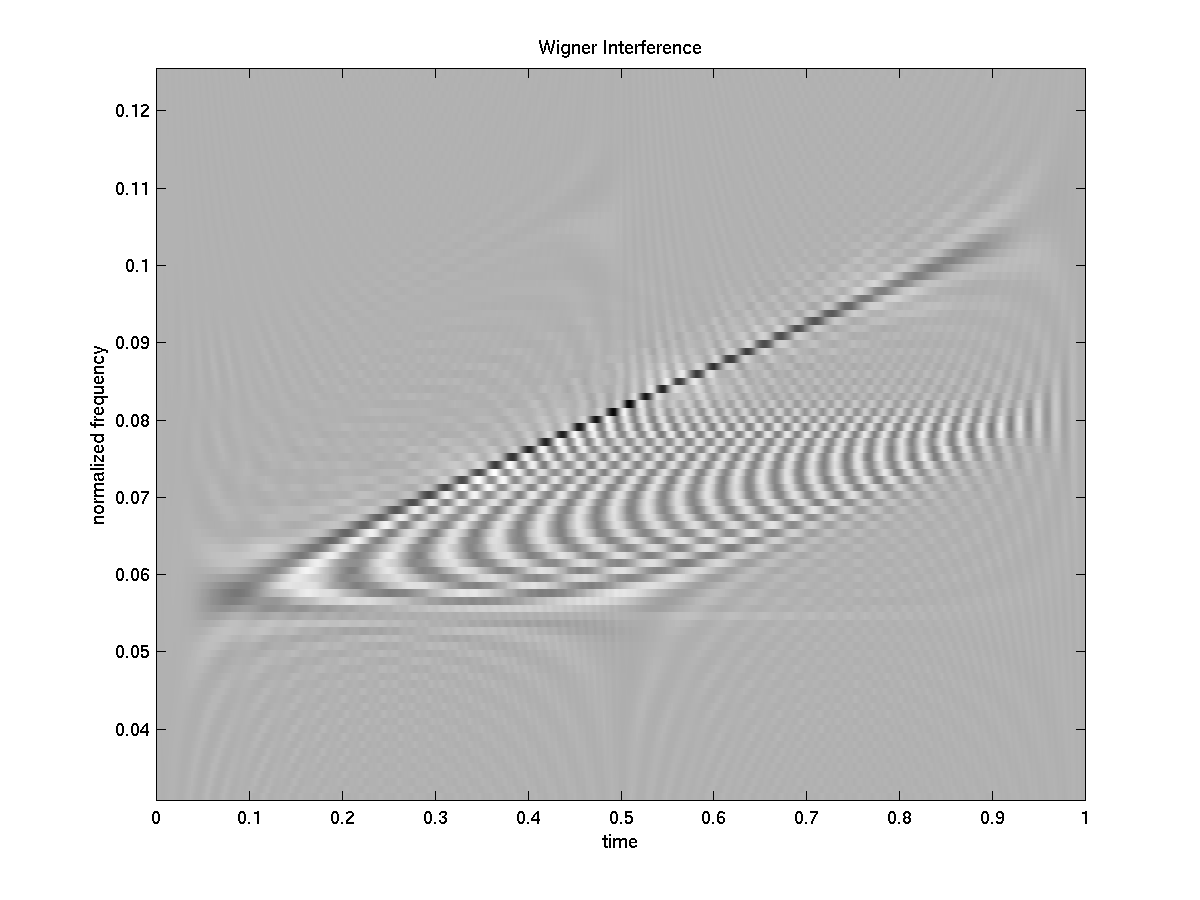
\includegraphics[width=7cm, height=6cm]{WVI}}
\caption{Wigner-Ville interference energy of a constant
  frequency modulation plus a linear chirp.}
\label{fig:WVI}
\end{center}
\end{figure}

\begin{figure}[htbp]
  \begin{center}
    \framebox[7cm]{\rule[-5mm]{0cm}{5cm}
  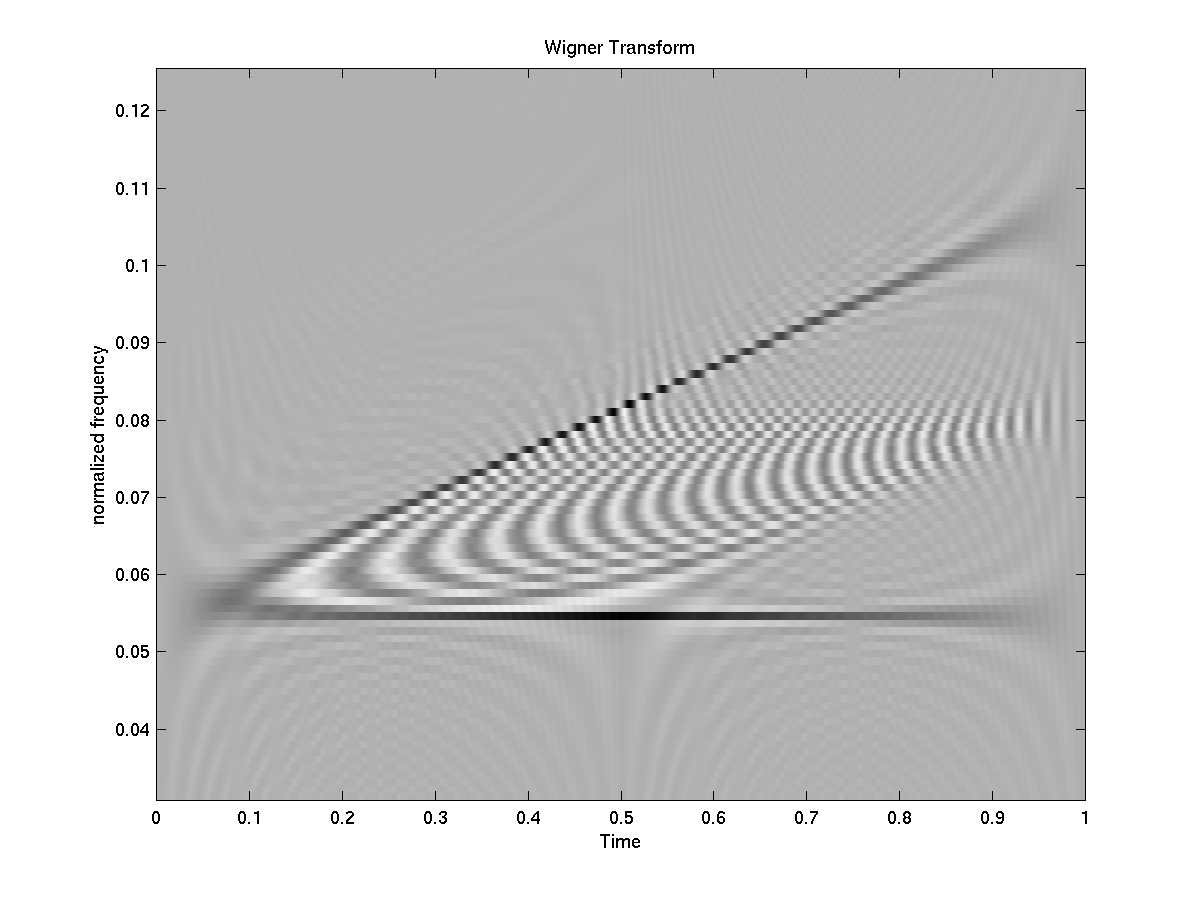
\includegraphics[width=7cm, height=6cm]{WVT}}
\caption{Wigner-Ville transform of a constant
  frequency modulation plus a linear chirp.}
\label{fig:WVT}
\end{center}
\end{figure}
}

The next section describes how we use the interference energy to derive a dissonance
measure of the signal.

\section{Dissonance Measures}
\def\tpull{\left(t+\halftau\right)}
\def\tpush{\left(t-\halftau\right)}
\def\I{\mathcal{I}}
\subsection{A Simple Dissonance Measure}
We first consider perhaps the simplest of the many possible dissonance measures
based on the information provided by the interference energy of the Wigner
transform. 

%Consider the function $\phi_{g_(\gamma_n}g_{\gamma_n}}(t,\tau)
Section~\ref{sec:wigner} introduced the function
$\phi_x(t,\tau)$.  Let's generalize this slightly by defining
\[
\phi_{g_{\gamma_m}g_{\gamma_n}}(t,\tau) 
= g_{\gamma_m}\tpull g^*_{\gamma_n}\tpush
\]
By definition of the cross \WT\ in equation~(\ref{eqn:crossWigner}),
$\W_{g_{\gamma_m}g_{\gamma_n}}$ is the Fourier transform of 
$\phi_{g_{\gamma_m}g_{\gamma_n}}(t,\tau)$ 
%$\phi_{m,n}$ 
with respect to $\tau$.  Therefore, the inverse Fourier 
transform of $\W_{g_{\gamma_m}g_{\gamma_n}}$ is
$\phi_{g_{\gamma_m}g_{\gamma_n}}$. 
%$\phi_{m,n}$.  
That is,
\[
\int
\W_{g_{\gamma_m}g_{\gamma_n}}(t,\nu) e^{i2\pi\nu\tau}\;d\nu
= \phi_{g_{\gamma_m}g_{\gamma_n}}(t,\tau) 
\]
Suppose that, at any given point in time, we integrate
$\W_{g_{\gamma_m}g_{\gamma_n}}(t,\nu)$ over all frequencies, $\nu$.  This is
equivalent to evaluating $\phi_{g_{\gamma_m}g_{\gamma_n}}$ at $\tau = 0$:
\begin{align}
\int
\W_{g_{\gamma_m}g_{\gamma_n}}(t,\nu)\;d\nu
&=\phi_{g_{\gamma_m}g_{\gamma_n}}(t,0)\nonumber \\
&= g_{\gamma_m}(t)g^*_{\gamma_n}(t) \label{eq:intWV}
\end{align}

As a first proposal, we consider measuring the dissonance at time $t$ of the
signal $x$ by integrating the interference energy
$I_x(t,\nu)$ over all frequencies $\nu$.  The result %in the continuous case,
is 
\begin{equation}\label{eq:specialI}
\I_x(t) = \int I_x(t,\nu)\; d\nu
\end{equation}
\[
=\sum_{m, n}
    \langle R^mx,g_{\gamma_m}\rangle \langle R^nx,g_{\gamma_n}\rangle^*
      \int \W_{g_{\gamma_m}g_{\gamma_n}}(t,\nu)\; d\nu
\]
%\[
%=2\sum_m\sum_{n>m}
%     \Real\left[\langle R^mx,g_{\gamma_m}\rangle \langle R^nx,g_{\gamma_n}\rangle^*
%        g_{\gamma_m}(t) g^*_{\gamma_n}(t)\right]
%\]
%Below we will see a graph of this measure for our %basic, yet revealing 
%example consisting of a sine tone plus a linear chirp. 

The lower graph in
Figure~\ref{fig:sIequal} shows how the function $\I_x(t)$ behaves for the
constant tone plus linear chirp.  The top graph is there for reference and
represents the value of the instantaneous frequencies of the signal.
Figure~\ref{fig:sIjust} also shows the value of $\I_x(t)$ for the example signal.
However, in this figure the time axes are delimited by tick marks representing
just and Pythagorean tunings. Table~\ref{table:ratios} presents the frequency
ratios corresponding to these tick marks.

%\begin{figure}[htbp]
%  \begin{center}
%    \framebox[7cm]{\rule[-5mm]{0cm}{5cm}
%  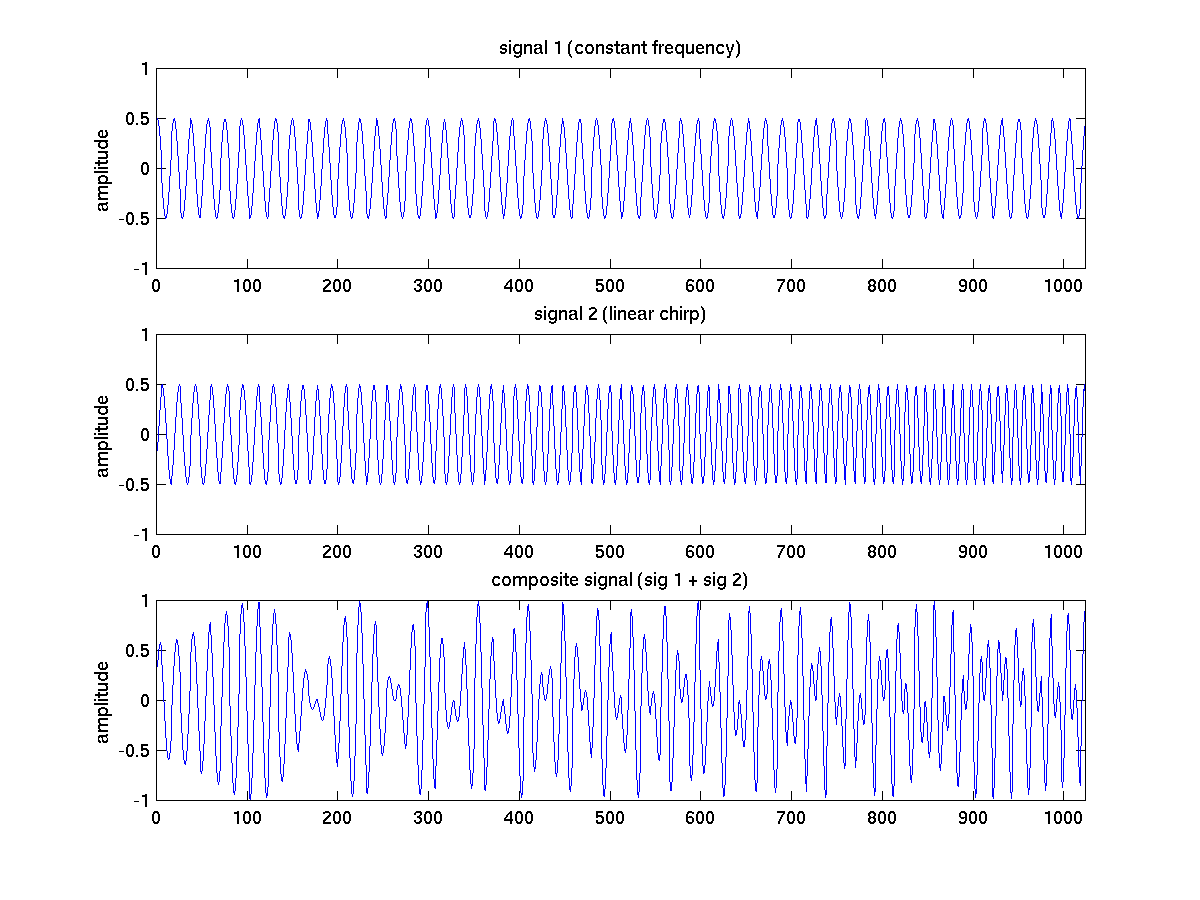
\includegraphics[width=7cm, height=6cm]{signal}}
%\caption{A constant frequency modulation plus a linear chirp.}
%\label{fig:signal}
%\end{center}
%\end{figure}

\ifthenelse{\boolean{nofigures}}{}{
\begin{figure}[htbp]
  \begin{center}
    \framebox[7cm]{\rule[-5mm]{0cm}{5cm}
  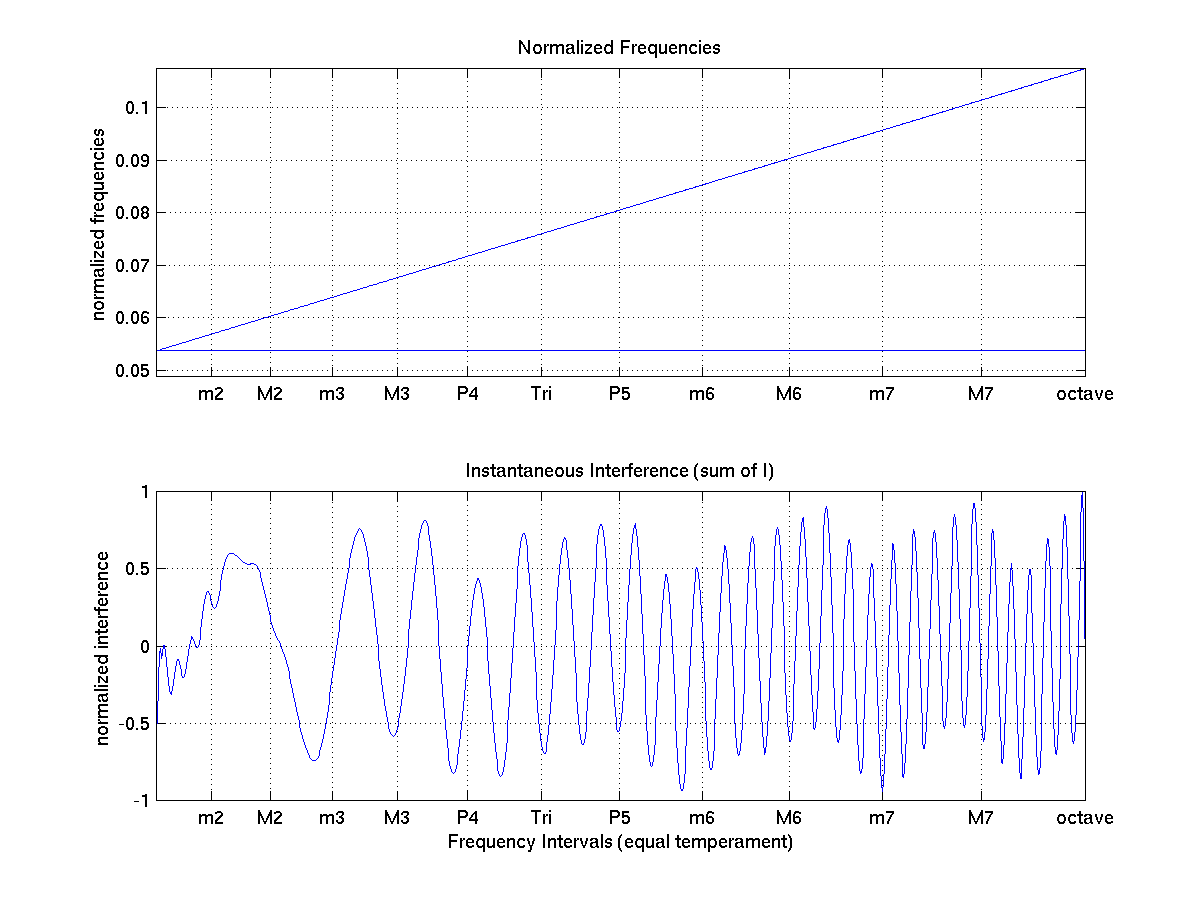
\includegraphics[width=7cm, height=6cm]{sumIequal}}
\caption{(a) Normalized instantaneous frequencies; (b) Instantaneous
  interference -- the sum of interferences at each point in time; the time
  axis of (b) is delimited by the ratio of the two frequencies in figure (a),
  with tick marks illustrating points of an equal tempered scale.}
\label{fig:sIequal}
\end{center}
\end{figure}
}
\begin{table}
  \begin{center}
%    \framebox[7cm]{\rule[-5mm]{0cm}{5cm}

\begin{tabular}{l|r|r|r}
Name & Just & Pythagorean & Equal\\
\hline
m2 &16/15& 256/243& $2^{1/12}$\\
M2 & 9/8 & 9/8& $2^{2/12}$\\
m3 &6/5 & 32/27& $2^{3/12}$\\
M3 &5/4 & 81/64& $2^{4/12}$\\
P4 &4/3 & 4/3& $2^{5/12}$\\
Tritone &64/45 & 729/512& $2^{6/12}$\\
P5 &3/2 & 3/2 & $2^{7/12}$\\
m6 &8/5&128/81& $2^{8/12}$\\
M6 & 5/3& 27/16 & $2^{9/12}$\\
m7 & 7/4& 16/9 & $2^{10/12}$\\
M7 & 15/8& 243/128 & $2^{11/12}$\\
octave& 2 & 2 & $2^{12/12}$
\end{tabular}
%}
\caption{Frequency ratios used to delimit the horizontal axis in the figures.}
\label{table:ratios}
\end{center}
\end{table}

\ifthenelse{\boolean{nofigures}}{}{
\begin{figure}[htbp]
  \begin{center}
    \framebox[7cm]{\rule[-5mm]{0cm}{5cm}
  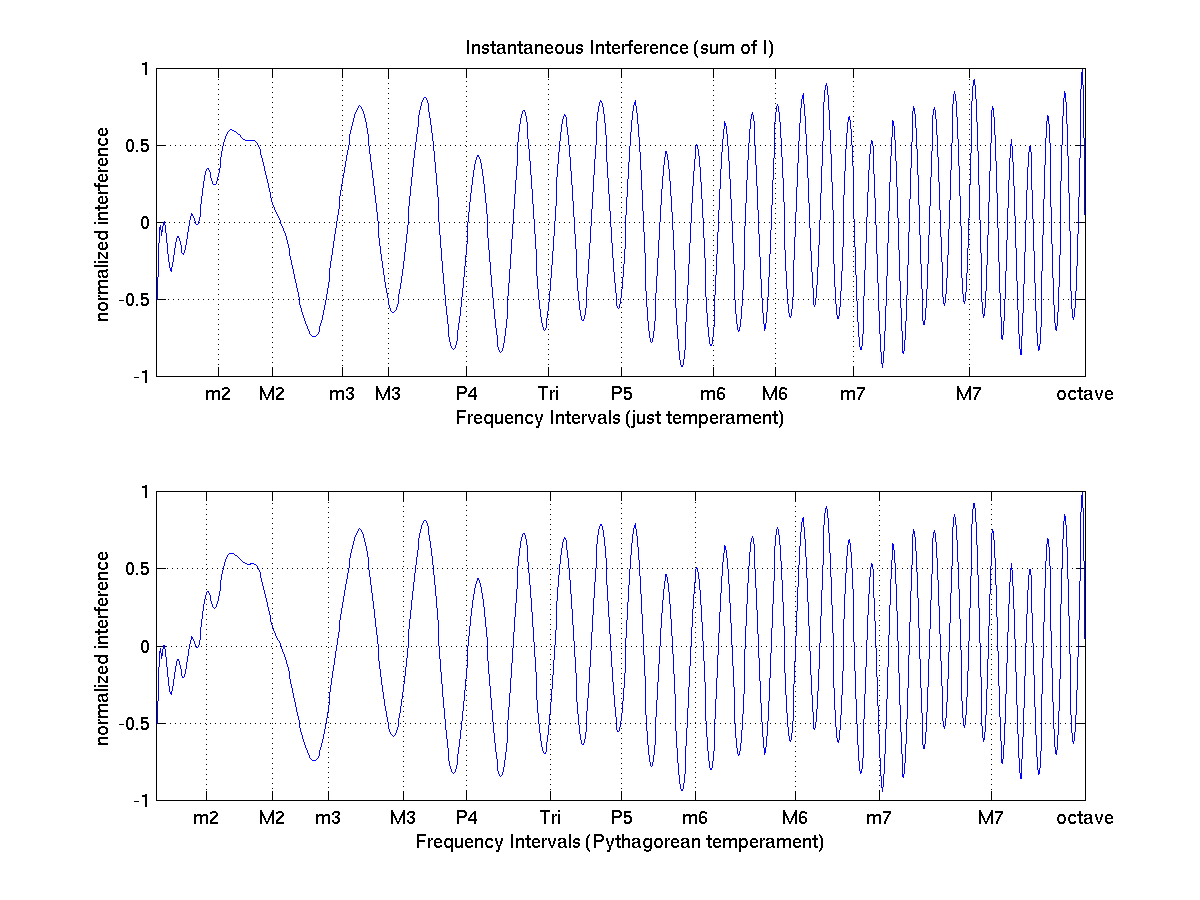
\includegraphics[width=7cm, height=6cm]{sumIjust}}
\caption{Instantaneous interference for just and Pythagorean tunings. This
  figure is the same as that of \ref{fig:sIequal} (b), except that the 
  tick marks illustrate points of a just (a) and Pythagorean (b) scale.}
\label{fig:sIjust}
\end{center}
\end{figure}
}

We first note that, in all three tuning systems, the perfect 5th falls in
roughly the same place, and that this interval consistently corresponds to
local minima of $\I_x(t)$. Other significant intervals, such as the major 3rd
and the tritone, also correspond to local minima of $\I_x(t)$.

\subsection{A General Dissonance Measure}
As stated at the outset, we want to find not only a point-wise measure of
dissonance, but also a measure that could account for melodic context.  The
function $\I_x(t)$ is essentially the sum over $\nu$ of the 
function $I_x(t,\nu)$.  Since $I_x(t,\nu)$ is a measure of interferences among
signal components centered at $t$ as well as those centered at times
surrounding $t$, it might seem as though the function $\I_x(t)$ accounts for
melodic context.  
However, note that
\[
\I_x(t) =\sum_{m,n}
      \langle R^mx,g_{\gamma_m}\rangle \langle R^nx,g_{\gamma_n}\rangle^*
        g_{\gamma_m}(t) g^*_{\gamma_n}(t)
\]
by equation~(\ref{eq:intWV}).
Thus $\I_x(t)$ only measures interferences among signal components at the
single time instant $t$. %, and it does not account for interferences occuring
%between atoms at different instances.  
Still, as the results for our simple example show, it may provide a useful
point-wise dissonance characterization of a signal.

We can generalize the foregoing by considering the inverse Fourier transform
of the interference energy:
%\begin{align*}
%\I_x(t,\tau) &= \int I_x(t,\nu)e^{i2\pi\nu\tau}\; d\nu\\
%&=\sum_{m, n} 
%\langle R^mx,g_{\gamma_m}\rangle \langle R^nx,g_{\gamma_n}\rangle^* \times\\
%&\quad \int \W_{g_{\gamma_m}g_{\gamma_n}}(t,\nu)e^{i2\pi\nu\tau}\; d\nu
%\end{align*}
%\end{align*}
%This is equivalent to
%\[
%\I_x(t,\tau) =\sum_{m, n} 
%\langle R^mx,g_{\gamma_m}\rangle \langle R^nx,g_{\gamma_n}\rangle^* 
%\phi_{g_{\gamma_m}g_{\gamma_n}}(t,\tau)
%\]
\[  
\I_x(t,\tau) = \int I_x(t,\nu)e^{i2\pi\nu\tau}\; d\nu  
\]
\[
= \sum_{m, n}\langle R^mx,g_{\gamma_m}\rangle \langle R^nx,g_{\gamma_n}\rangle^* 
\phi_{g_{\gamma_m}g_{\gamma_n}}(t,\tau)
\]
Recall,
\[
\phi_{g_{\gamma_m}g_{\gamma_n}}(t,\tau) 
= g_{\gamma_m}\tpull g^*_{\gamma_n}\tpush
\]
The function $\I_x(t,\tau)$ leads to dissonance measures based on interferences
between signal components at different points in time.  For instance, a measure
of interferences among signal components that are separated by not more than 
$\tau_0$ units of time is
\begin{align}\label{eq:indicatorDiss}
\I_x^{\tau_0}(t) &= \int_0^{\tau_0} \I_x(t,\tau)\; d\tau\\
&=\sum_{m, n} \langle R^mx,g_{\gamma_m}\rangle \langle
                      R^nx,g_{\gamma_n}\rangle^* \times \nonumber\\
&\quad \int_0^{\tau_0} g_{\gamma_m}\tpull g^*_{\gamma_n}\tpush\;d\tau\nonumber
\end{align}
Of course, we can vary $\tau_0$ depending on the extent to which we wish to
account for interferences among signal components across time. 

More generally, put a distribution $\mu$ on the domain of time differences
among signal components.  This distribution describes the
relative importance of the interferences across various time intervals.  Then define,
\begin{equation}\label{eq:generalDiss}
\I_x^{\mu}(t) = \integral \I_x(t,\tau)\; d\mu(\tau)
\end{equation}

The definition of $\I_x$ in equation~(\ref{eq:specialI}) and $\I_x^{\tau_0}$
in equation~(\ref{eq:indicatorDiss}) are special cases
of~(\ref{eq:generalDiss}). We arrive at $\I_x^{\tau_0}$ by setting
\[
d\mu(\tau) = \chi_{[0,\tau_0)}(\tau)\;d\tau
\]
where $\chi_{[0,\tau_0)}(\tau)$ is the characteristic function, equal to 1 when
$\tau \in [0,\tau_0)$ and 0 elsewhere. In this case, $\mu$ is a uniform
distribution of width $\tau_0$.  Therefore, $\mu$ assigns equal importance to
interferences among components separated by at most $\tau_0$ units of time,
and zero importance to interferences among components separated by more than
$\tau_0$ units. Clearly, by setting $\tau_0 = 0$ in the foregoing, we
  return to the simplest measure, $\I_x$, with which we began.

Figure~\ref{fig:Icorr} shows how the function $\I_x^{\tau_0}$ behaves for our
example signal and two values of $\tau_0$.  The upper graph shows
$\I_x^{\tau_0}$ for $\tau_0 = 5.9$ milliseconds, and the lower graph shows
the same function for $\tau_0 = 46.9$ milliseconds.  

One interesting aspect of these figures is the behavior they exhibit near
the perfect fifth interval.  Taken as a measure of dissonance, the figures
indicate that dissonance is high when the ratio approaches the perfect fifth
and low once it reaches the perfect fifth. 
%In fact, for $\tau_0 = 46.9$
%milliseconds, the perfect fifth acheives minimum dissonance.

\ifthenelse{\boolean{nofigures}}{}{
\begin{figure}[htbp]
  \begin{center}
    \framebox[7cm]{\rule[-5mm]{0cm}{5cm}
  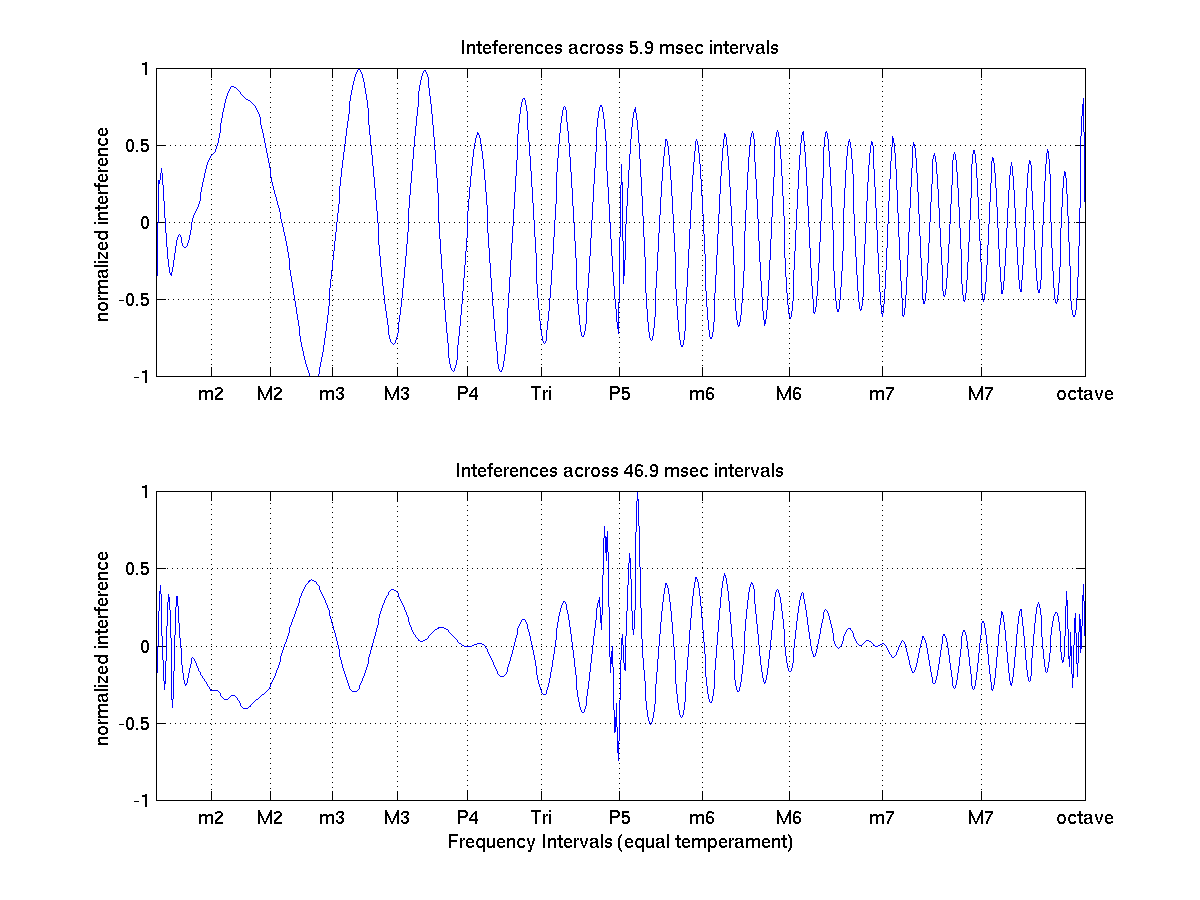
\includegraphics[width=7cm, height=6cm]{IcorrEqual}}
\caption{Interference measure $\I_x^{\tau_0}$; the sum of interferences over
  the given time intervals.}
\label{fig:Icorr}
\end{center}
\end{figure}
}

\section{Conclusion}
We have described the function, $I_x$, representing the sum of the
interference terms of the \WT\ of a signal. %, and we called this the
%interference energy of the signal.  
Based
on this function we derived a measure, $\I_x^{\tau_0}$, of interference among
signal components over a given interval of time, $\tau_0$.  Finally, we
proposed a general interference measure, $\I_x^{\mu}$, by putting a distribution
$\mu$ on the domain of time differences between signal components.  

The dissonance measure that results from the foregoing depends on the function
$\mu$, which represents the relative importance we place on interferences
across various time intervals.  Generalizing $\I_x$ is this way enables
the interference function to account for melodic context, and this provides
heuristic justification for the use of $\I_x^{\mu}$ as a measure of melodic
dissonance.

We have shown that the measures presented above exhibit interesting
behavior for our simple example.  However, it is as yet unclear exactly how
useful, as measures of dissonance,  %is the information provided by 
are such functions.  We expect that further research, and experience with
these functions in musical situations, will at least demonstrate their utility
as a means of characterizing musical signals.   

%%% Local Variables: 
%%% mode: latex
%%% TeX-master: "ICMC"
%%% End: 
